\documentclass[12pt]{article}

\usepackage{amssymb,amsmath,amsthm} % Include AMS Math symbols
\usepackage{graphicx}               % Allows for importation of figures 
\usepackage{float} % to get the table where i want it
\usepackage{booktabs} % professional table typesetting commands 

\usepackage{color}   % Sets up a nice typesetting environment for Python
\usepackage{listings}
\definecolor{dkgreen}{rgb}{0,0.6,0}
\definecolor{gray}{rgb}{0.5,0.5,0.5}
\definecolor{mauve}{rgb}{0.58,0,0.82}
\lstset{frame=tb,
  language=Python,
  aboveskip=3mm,
  belowskip=3mm,
  showstringspaces=false,
  columns=flexible,
  basicstyle={\small\ttfamily},
  numbers=left,
  numberstyle=\tiny\color{gray},
  keywordstyle=\color{blue},
  commentstyle=\color{dkgreen},
  stringstyle=\color{mauve},
  breaklines=true,
  breakatwhitespace=true,
  tabsize=3
}

% define command \expandableinput  for table input
\makeatletter
\def\expinput#1{\@@input#1 }
\makeatother

\title{ HW \# 2\\ Math/CS 471, Fall 2026}
\author{Theo Nichols \\ Andrew Vargas}
\date{September 15, 2026}   % Activate to display a given date or no date


\begin{document}

% Display title
\maketitle
\clearpage

\section{Part 1: One Dimensional Newton's Method}

\subsection{Description}
We are tasked with finding the roots of three different scalar functions and determining the convergence rate, or rate at which our computational methods approach the root. Two of these are non-linear, and one is a simple linear function, the importance of which will be explored in subsequent sections. We are provided the Python code for and instructed to use Newton's Method, an iterative method which uses an initial guess for a root, or zero, of the function, and then repeats the formula below, where $x_{n+1}$ is the new guess for the root, $x_n$ is the previous, $f$ refers to the function, and $f'$ its derivative.
\begin{equation*}
    x_{n+1} = x_n - \frac{f(x_n)}{f'(x_n)}
\end{equation*}

\subsection{Method}
We used the provided code, and made some simple modifications to determine the convergence rate of Newton's Method, as well as place safeguards that ensure the code would iterate an appropriate number of times or halt if it would otherwise iterate indefinitely. To accomplish that, we simply added a user defined tolerance for the error estimate, and a maximum number of iterations that if reached would likely imply Newton's method was going to fail to find a root. Of course, this involved calculating an approximation of the error at each iteration. Our error estimate was calculated as $|x_{n+1} - x_n|$. \\ \\If this value  was found to be less than the user defined tolerance, the code would break. We were advised to choose $10^{-10}$ as our tolerance, and a maximum number of iterations that would give the method time to converge. I chose 100 rather arbitrarily, and this number of iterations was never reached. \\ \\We then calculated the convergence rate. The convergence rate refers to the rate at which a method approaches a true root. We tested for linear and quadratic convergence, where linear convergence implies that the error of the next iteration is proportional to a constant times the error of the current error, and quadratic convergence is more rapid as the error at the next step is proportional to the square of the current error.
To calculate the convergence rate, we took the ratio of the error estimate for the next iteration divided by that of the previous iteration. We first populated an array with these error estimates, then simply calculated $\frac{errors[i+1]}{errors[i]}$ and $\frac{errors[i+1]}{errors[i]^2}$ for linear and quadratic convergence respectively.\\ 
\\If a ratio remained nearly constant for every iteration, this implied the method was converging at that rate, as the errors were proportional. If on the other hand the values continued to change, this meant the errors were not proportional and the method was not converging at that rate. Below is a snippet of our Python code for computing these ratios. 
\begin{verbatim}
k_l = 0
k_q = 0
errors = []

for i in range(len(data) - 1):
    errors.append(abs(data[i+1] - data[i]))

for i in range(len(errors) -1):
    k_l = errors[i+1] / errors[i]
    k_q = errors[i+1] / (errors[i]**2)
        
    print("Linear convergence ration: " + str(k_l))
    print("Quadratic convergence ration: " + str(k_q))

\end{verbatim}
Data was an array containing all of the potential roots generated by the newton.py file provided to us. We piped the output of this driver code into a text file and the results can be seen in Table 1 below.

\begin{table}[H]
\centering
\begin{tabular}{c|c|c}
\toprule
Function & Linear Ratio & Quadratic Ratio \\
\midrule
$f(x)=x^2$ 
\expinput{convergence_1.txt}
\midrule
$f(x)=\sin(x)+\cos(x^2)$
\expinput{convergence_3.txt}
\bottomrule
\end{tabular}
\caption{Functions and Their Computed Convergence Ratios}
\label{tab:1}
\end{table}

\subsection{Interpretation} 
As can be seen in Table 1, the linear ratio for $f(x) = x^2$ remained a constant 0.5. This indicates that Newton's did indeed converge linearly for this particular function and initial guess. The reason this occurs is due to the behavior of $f'(x)$ near the root. \\\\If we rewrite Newton's Method, $x_{n+1} = x_n - \frac{f(x_n)}{f'(x_n)}$ using the function \\$f(x) = x^2$, we get $x_n - \frac{x^2_n}{2x_n} = x_n - \frac{1}{2}x_n = \frac{1}{2}x_n$ which is precisely the definition of linear convergence, as the error is decreasing by a constant factor at each step. The root encountered here is a multiple root, that is, the function touches zero here but then rebounds in the positive y direction. The quadratic ratio continues to grow, indicating that the error is not proportional to the square of the error at each step. \\\\For $f(x) = x$, the reason there is no data is due to the fact that it is a linear function. As a result, Newton's method converges in one step, that is, with an initial guess of -0.5, the first computation yields \\$f(-0.5) - \frac{f(-0.5)}{f'(-0.5)} = -0.5 - -0.5 = 0$. As such there is no error, and the actual root of $x = 0$ has been found in a single step. \\ \\For $f(x) = sin(x) + cos(x^2)$, the linear ratio does not remain constant, but the quadratic ratio remains nearly constant, thus indicating quadratic convergence. The anomalous last value occurs because as Newton's Method gets closer to the root, the error becomes very small. Since the quadratic ratio divides the next error by the square of the current error, squaring an already very small error produces an extremely small denominator, causing the ratio to become very large. This does not indicate that the method is not converging quadratically, but is the result of a lack of numerical precision on my machine.

\clearpage

\section{Part 2: Multi-Dimensional Newton's Method}
\subsection{Description}
In part 2, we are tasked with extending Newton's Method from solving a single nonlinear equation to solving a system of nonlinear equations that models the electrical network as shown in lecture. We consider the electrical network shown in Figure \ref{fig: sample_eletrical_network} and the corresponding adjacency matrix $A$, which is $m$ x $n$ for $m$ = 8 edges and $n$ = 6 nodes in part 1, and $m$ = 10 and $n$ = 7 for part 2. \\
\begin{figure}[H]
\centering
\includegraphics[width=0.75\textwidth]{fig1_sample_electrical_network.png}
\caption{A graph of the network in part 1 of question 2.}
\label{fig: sample_eletrical_network}
\end{figure}
\newcommand{\p}{\phantom{-}}
\[
A = 
\begin{bmatrix} 
{-1} & \p0 & \p0 & \p1 & \p0 & \p0\\
\p0 & \p0 & \p0 & {-1} & \p1 & \p0\\
\p0 & \p0 & \p0 & \p0 & {-1} & \p1\\
\p0 & \p0 & \p1 & \p0 & \p0 & {-1}\\
\p0 & \p1 & {-1} & \p0 & \p0 & \p0\\
\p1 & {-1} & \p0 & \p0 & \p0 & \p0\\
\p0 & {-1} & \p0 & \p0 & \p0 & \p1\\
\p0 & \p0 & \p0 & {-1} & \p0 & \p1
\end{bmatrix}
\]
\\\\
Using our 1D Newton's code as a guide, we solve for a vector v containing the unknown voltages at each node in the network. \\\\
The network will be represented by a matrix, $A$, and a source vector, $s$. $A$  will describe how the nodes are connected. $s$ will represent the external current entering and leaving the system. The voltage differences across the edges are given by $Av$. The admittance of each edge is modeled as a nonlinear function of these voltage differences. 
The nonlinear admittance is defined by
$$
\widetilde{y}(d)=\frac{Y}{1+\alpha d^2},
$$
where \(Y\) is the base admittance and \(\alpha\) controls how strongly the admittance changes with the voltage difference \(d\). Thus, the current through each edge is given by
$$
I_j=\widetilde{y}(d_j)d_j.
$$
The resulting nonlinear system can therefore be written as
$$
f(v)=A^T\operatorname{diag}(\widetilde{y}(Av))Av-s.
$$
\\\\ 
The resulting nonlinear system is written in the form \begin{equation}f(v) = 0.
\end{equation} Multidimensional Newton's Method is used to approximate the node voltages that satisfy the system. \\\\
This process is carried out in two different networks. The convergence behavior of Newton's Method is examined for each electrical network. 

\subsection{Method}
Here we will explain the driver code that sets up the electrical network and applies multidimensional Newton's method to solve for the node voltages.

The first network connectivity of the system was represented using the 8 x 6 matrix $A$, corresponding to eight edges and six nodes. The source vector was defined as \begin{equation} s = [1, -1, 0, 0, 0, 0,]^T \end{equation} and its entries sum to zero, satisfying the current-balance requirement for the network. The nonlinear admittance parameters are set to \begin{equation} Y = 1 \end{equation} and \begin{equation} \alpha = 0.5.\end{equation} For a vector of node voltages $v$, the voltage differences across the network edges were calculated using \begin{equation} d = Av. \end{equation} The nonlinear admittance of each edge was then evaluated using \begin{equation}
    \tilde{y}(d) = \frac{Y}{1 + \alpha d^2},
\end{equation}
and its derivative was computed as 
\begin{equation}
    \tilde{y}'(d) = \frac{-2 \alpha d Y}{(1 + \alpha d^2)^2}.
\end{equation}
These quantities were used to construct the nonlinear system \begin{equation}
    f(v) = A^T diag(\tilde{y}(Av))Av - s,
\end{equation}
whose root corresponds to a set of node voltages that satisfies the network equations. 
\\\\
To apply multidimensional Newton's method, the Jacobian of $f(v)$ was also required. For each voltage vector $v$, the edge voltage differences $d = Av$ were first calculated, followed by $\tilde{y}(d)$ and $\tilde{y}'(d)$. Then a diagonal matrix $K$ was constructed with the diagonal entries \begin{equation}
    K_{jj} = \tilde{y}(d_j) + \tilde{y}'(d_j)d_j.
\end{equation}
The Jacobian was subsequently formed as 
\begin{equation}
    J_f(v) = A^TKA.
\end{equation}
Since $A^T$ has dimensions 6 x 8, $K$ has dimensions 8 x 8, and $A$ has dimensions 8 x 6. The resulting Jacobian matrix is 6 x 6, corresponding to the six unknown node voltages. The Python implementation followed this expression directly using \verb|A.T @ K @ A|. 
\\\\
An additional issue arises because the network formulation does not uniquely determine an absolute voltage reference. Rather, the equations depend on voltage differences between nodes. As a result, the matrix used to form the initial approximation is singular and cannot be inverted using an ordinary matrix inverse. 
\\\\
To account for this, the Moore-Penrose pseudoinverse was used through the NumPy's \verb|np.linalg.pinv()| function, in both the formulation of the initial guess and subsequent iterations. 
The prescribed initial guess was formed from \begin{equation}
    v^{0} = [A^T diag(\tilde{y}(0))A]^\dagger s.
\end{equation}
Since $\tilde{y}(0) = 1$, the initial edge admittances are all equal to one. In the code, an eight entry zero vector was first used to evaluate $\tilde{y}(0)$, after which the matrix $A^T diag(\tilde{y}(0))A$ was constructed. Its pseudoinverse was multiplied by $s$ to obtain
\[
v^{(0)} \approx 
\begin{bmatrix}
\p 0.41667\\
-0.28333\\
-0.18333\\
\p 0.11667\\
\p 0.01667\\
-0.08333
\end{bmatrix}
.\]

This vector was then supplied as the starting approximation for multidimensional Newton's method.

\subsection{Interpretation} 
Below we will discuss the results of our implementation of multidimensional Newton's method by providing the convergence data and diagrams of the network solutions.

\begin{table}[H]
\centering
\begin{tabular}{c|c}
\toprule
Newton Iteration $k$ & $\|f(v^{(k)})\|_2$ \\
\midrule
\expinput{multiNewtonIters.txt}
\bottomrule
\end{tabular}
\caption{Values of $\|f(v^{(k)})\|_2$ for Newton's method}
\label{tab:1}
\end{table}

To examine the convergence rate, the quadratic convergence ratio was computed as
$$
\frac{\|f(v^{(k+1)})\|}{\|f(v^{(k)})\|^2}.
$$
For the successive iterations, these ratios are
$$
\frac{0.021152057}{(0.20733047)^2}
\approx 0.492,
$$
$$
\frac{0.00031984797}{(0.021152057)^2}
\approx 0.715,
$$
$$
\frac{7.6644545\times10^{-8}}
     {(0.00031984797)^2}
\approx 0.749,
$$
and
$$
\frac{4.3261986\times10^{-15}}
     {(7.6644545\times10^{-8})^2}
\approx 0.736.
$$
The ratio becomes approximately constant as the iteration progresses, with the final three values all near \(0.74\). This behavior indicates that Newton's method exhibits quadratic convergence as it approaches the solution. The residual norm also decreases every iteration, and therefore the method converges monotonically.

\begin{table}[H]
\centering
\begin{tabular}{c|c}
\toprule
Newton Iteration $k$ & $\|f(v^{(k)})\|_2$ \\
\midrule
\expinput{multiNewtonIters2.txt}
\bottomrule
\end{tabular}
\caption{Values of $\|f(v^{(k)})\|_2$ for Newton's method}
\label{tab:1}
\end{table}

To examine the convergence rate, the quadratic convergence ratio was computed as
$$
\frac{\|f(v^{(k+1)})\|}{\|f(v^{(k)})\|^2}.
$$
For the final iterations, these ratios are
$$
\frac{9.2951513\times10^{-7}}
     {(2.0884397\times10^{-3})^2}
\approx 0.213,
$$
and
$$
\frac{1.8450049\times10^{-13}}
     {(9.2951513\times10^{-7})^2}
\approx 0.214.
$$
Since these values are approximately constant, the residuals exhibit quadratic convergence, as expected for Newton's method near the solution. As the residual norm decreases every iteration, the method converges monotonically. \\

Below are graphical representations of the solutions to the networks in both parts of problem 2. \\
\begin{figure}[H]
\centering
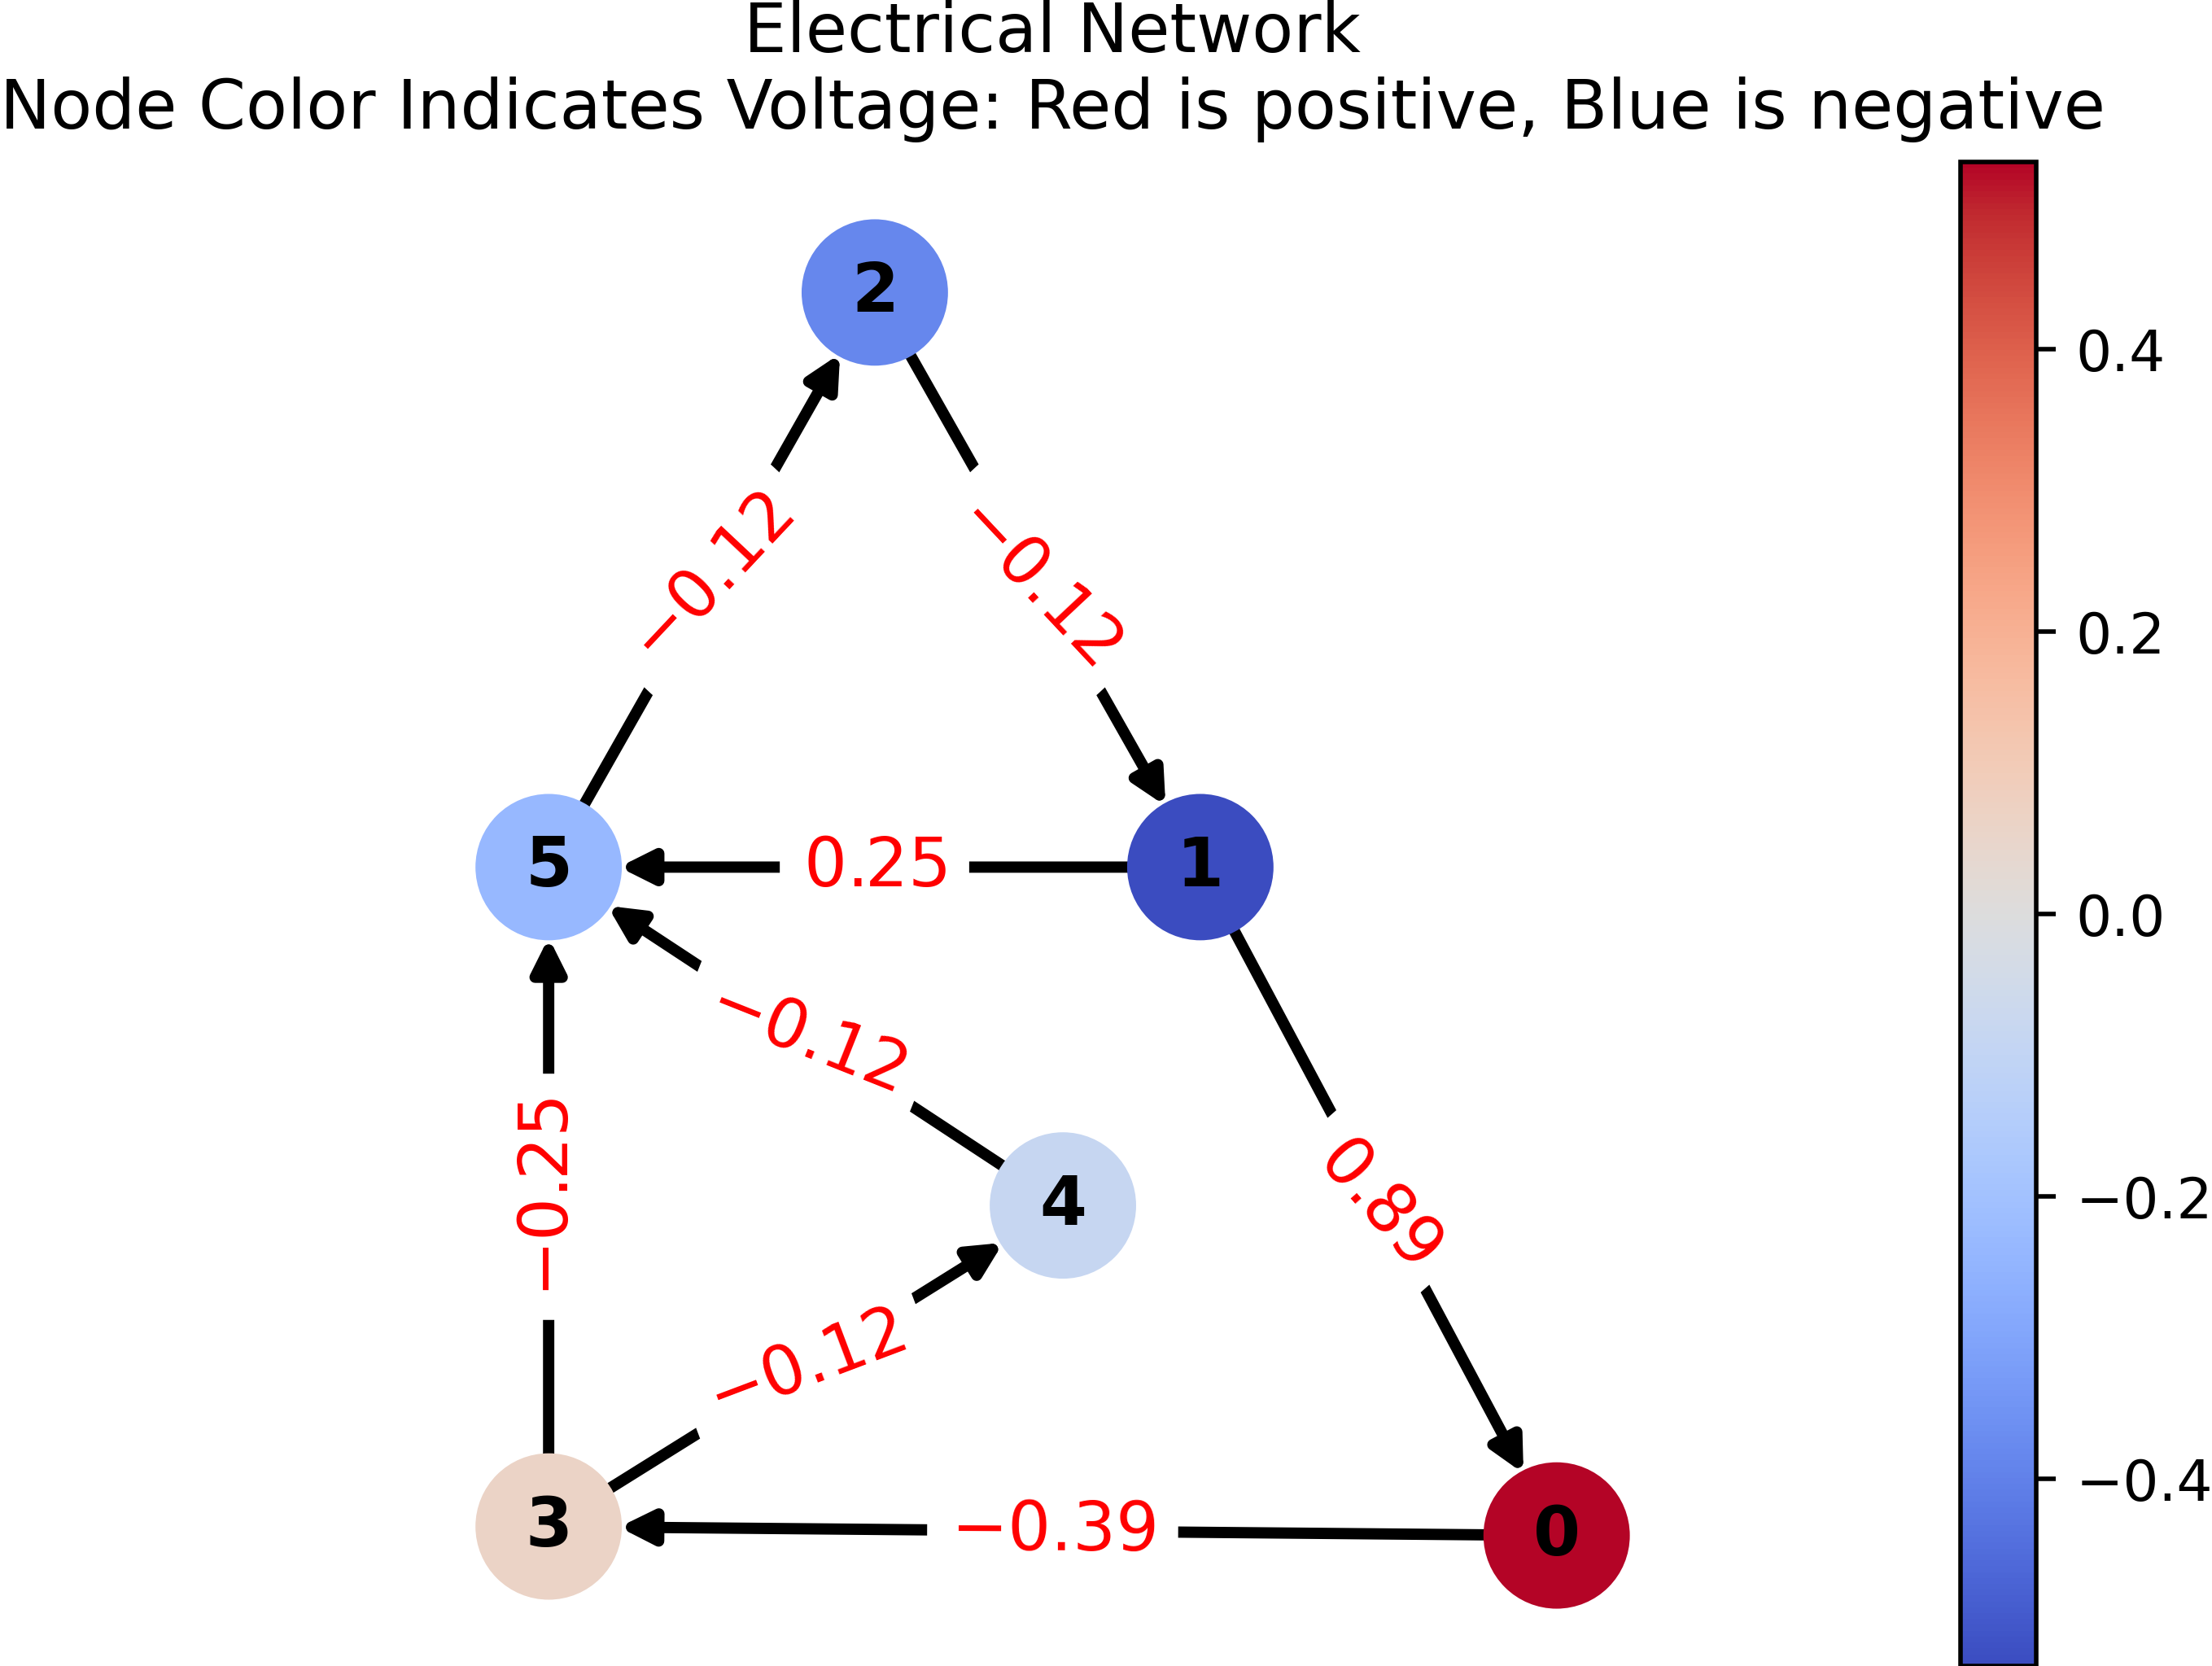
\includegraphics[width=0.75\textwidth]{network_solution.png}
\caption{This figure displays the solution to the network provided in part 1 of question 2.}
\label{fig:network_solution}
\end{figure}
\begin{figure}[H]
\centering
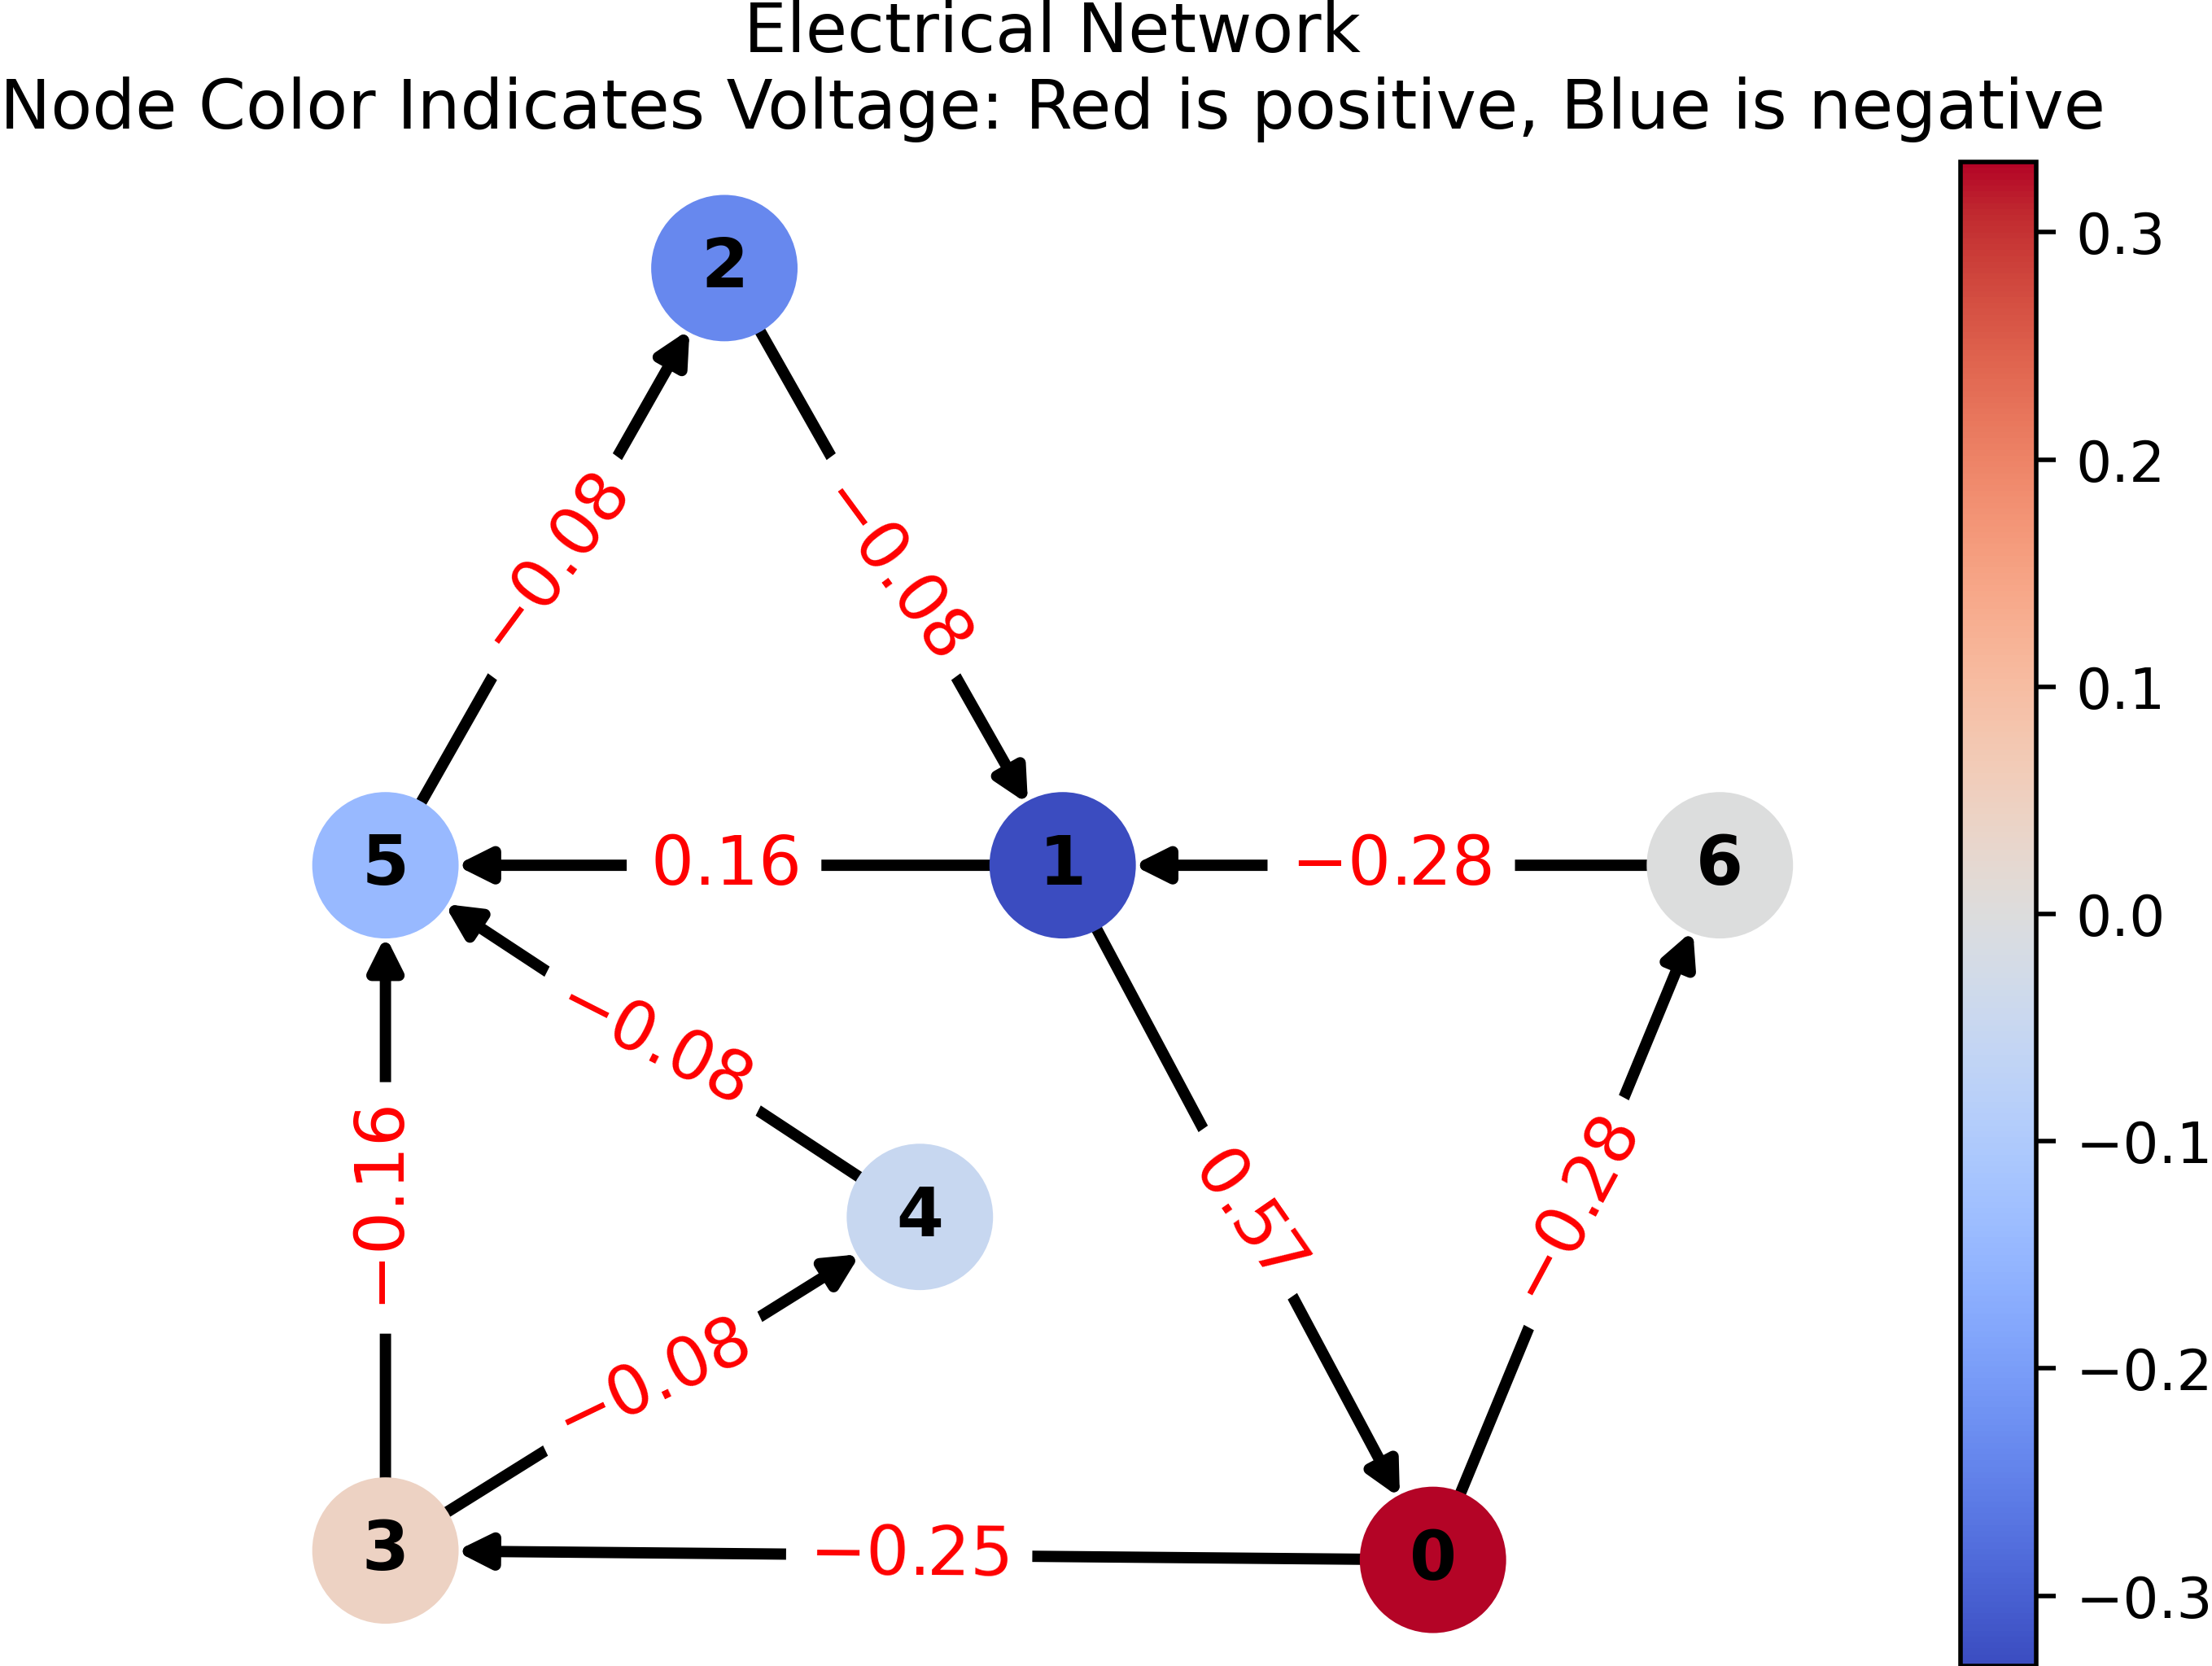
\includegraphics[width=0.75\textwidth]{network_solution2.png}
\caption{This figure displays the solution to the network provided in part 2 of question 2.}
\label{fig:network_solution2}
\end{figure}

As can be seen in both figures, a solution has been found that satisfies both Kirchhoff and Ohm's law. Something interesting of note occurs at node 6. Here, Kirchhoff's Current Law is satisfied because the incoming and outgoing currents are both approximately \(-0.28\). The negative signs indicate that the actual current directions are opposite the directions assigned by the adjacency matrix. Since the two signed currents are equal, their net contribution at node 6 is zero:
$$
-0.28-(-0.28)=0.
$$
Because there is no external current source at node 6 (\(s_6=0\)), this satisfies Kirchhoff's law and confirms that the current is conserved at the node.

\end{document}  
